\documentclass[12pt]{article}
\usepackage{fullpage, amsmath, amssymb, amsthm, amscd, setspace, bm, graphicx, indentfirst, multirow, tikz, enumerate, verbatim, appendix}

\usepackage{adjustbox,amsfonts,array,graphicx,booktabs,tabularx,multirow,multicol,stmaryrd, tabu}
\usepackage[utf8]{inputenc}
\usepackage{cite}
\usepackage{hyperref}
\usetikzlibrary{arrows.meta}
\title{Math 412, Fall 2023 -- Homework 1}
\date{}
\setlength{\parskip}{0.5cm}
\setlength{\parindent}{0cm}

\newtheorem{theorem}{Theorem}[section]
\newtheorem{definition}[theorem]{Definition}
\newtheorem{lemma}[theorem]{Lemma}
\newtheorem{proposition}[theorem]{Proposition}
\newtheorem{corollary}[theorem]{Corollary}
\newtheorem{remark}[theorem]{Remark}
\newtheorem{example}[theorem]{Example}

\newcommand{\Z}{\mathbb{Z}}
\newcommand{\R}{\mathbb{R}}
\newcommand{\Q}{\mathbb{Q}}
\newcommand{\C}{\mathbb{C}}
\newcommand{\F}{\mathbb{F}}
\newcommand{\N}{\mathbb{N}}
\newcommand{\U}{\mathcal{U}}
\newcommand{\B}{\mathcal{B}}
\newcommand{\T}{\mathbb{T}}
\newcommand{\real}{\textrm{Re }}
\newcommand{\imag}{\textrm{Im }}
\newcommand{\deriv}[2]{\frac{d #1}{d #2}}
\newcommand{\sig}[1]{\sum_{#1 =1}^\infty}
\newcommand{\un}[1]{\bigcup_{#1 =1}^\infty}
\newcommand{\inter}[1]{\bigcap_{#1 =1}^\infty}
\newcommand{\cyc}[2]{\genfrac{[}{]}{0pt}{}{#1}{#2}}
\newcommand{\px}[2]{\genfrac{\{}{\}}{0pt}{}{#1}{#2}}
\newcommand{\wh}[1]{\widehat{#1}}
\newcommand{\del}{\partial}
\newcommand{\st}{ \; \big | \:}
\newcommand{\ba}{\overline}
\newcommand{\Int}{\mathrm{Int}}
\newcommand{\Cl}{\mathrm{Cl}}
\newcommand{\rel}{\mathrm{rel}}
\newcommand{\Hom}{\text{Hom}}
\newcommand{\End}{\text{End}}
\newcommand{\Mor}{\text{Mor}}
\newcommand{\Ind}{\text{Ind}}
\newcommand{\Irr}{\text{Irr}}
\newcommand{\vect}[1]{\boldsymbol{#1}}
\newcommand{\mfk}[1]{\mathfrak{#1}}
\newcommand{\wt}{\text{wt}}
\newcommand{\vx}[1]{\mathtt{#1}}
%\renewcommand{\wt}[1]{\mathtt{#1}}
\begin{document} \maketitle
\vspace{-80pt}

\textbf{Due:} Wednesday, August 30th, at 9:00AM via Gradescope

\textbf{Instructions:} Students taking the course for three credit hours (undergraduates, most graduate
students) should choose four of the following five problems to solve and turn in--if you do all five, only the first four will be graded. Graduate students
taking the course for four credits should solve all five. Problems that use the word “describe”,
“determine”, "show", or "prove" require proof for all claims.

\begin{enumerate}
\item[1.] Of the following graphs, determine which pairs of graphs are isomorphic (and which are nonisomorphic).

\begin{center}
\scalebox{0.7}{
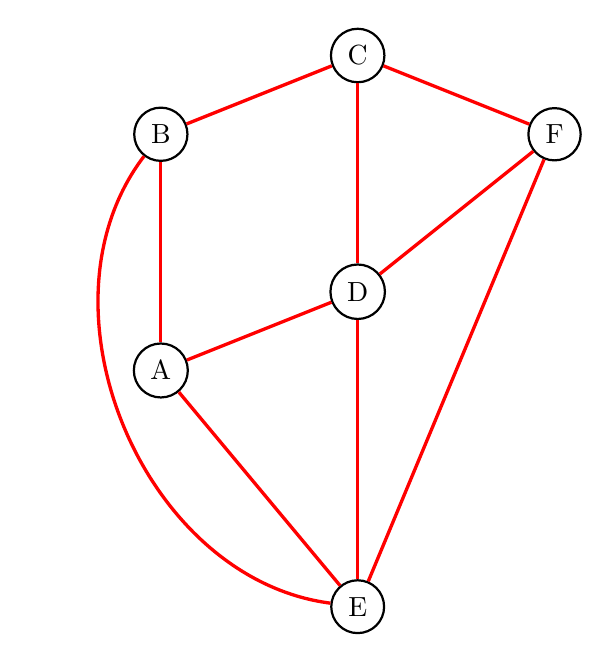
\begin{tikzpicture}
\begin{scope}[every node/.style={circle,thick,draw}]
    \node (A) at (0,0) {A};
    \node (B) at (0,3) {B};
    \node (C) at (2.5,4) {C};
    \node (D) at (2.5,1) {D};
    \node (E) at (2.5,-3) {E};
    \node (F) at (5,3) {F} ;
\end{scope}

\begin{scope}[>={Stealth[black]},
              every node/.style={fill=white,circle},
              every edge/.style={draw=red,very thick}]
    \path [-] (A) edge (B);
    \path [-] (B) edge (C);
    \path [-] (A) edge (D);
    \path [-] (D) edge (C);
    \path [-] (A) edge (E);
    \path [-] (D) edge (E);
    \path [-] (D) edge (F);
    \path [-] (C) edge (F);
    \path [-] (E) edge (F); 
    \path [-] (B) edge[bend right=60] (E); 
\end{scope}
\end{tikzpicture}
\hspace{50pt}
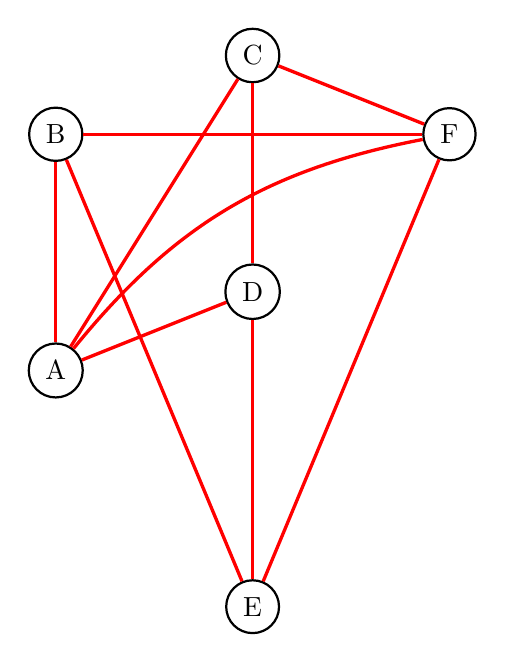
\begin{tikzpicture}
\begin{scope}[every node/.style={circle,thick,draw}]
    \node (A) at (0,0) {A};
    \node (B) at (0,3) {B};
    \node (C) at (2.5,4) {C};
    \node (D) at (2.5,1) {D};
    \node (E) at (2.5,-3) {E};
    \node (F) at (5,3) {F} ;
\end{scope}

\begin{scope}[>={Stealth[black]},
              every node/.style={fill=white,circle},
              every edge/.style={draw=red,very thick}]
    \path [-] (C) edge (D);
    \path [-] (D) edge (E);
    \path [-] (C) edge (F);
    \path [-] (F) edge (E);
    \path [-] (C) edge (A);
    \path [-] (F) edge[bend right=20] (A);
    \path [-] (F) edge (B);
    \path [-] (E) edge (B);
    \path [-] (A) edge (B); 
    \path [-] (D) edge (A); 
\end{scope}
\end{tikzpicture}}
\end{center}

\begin{center}
\scalebox{0.7}{
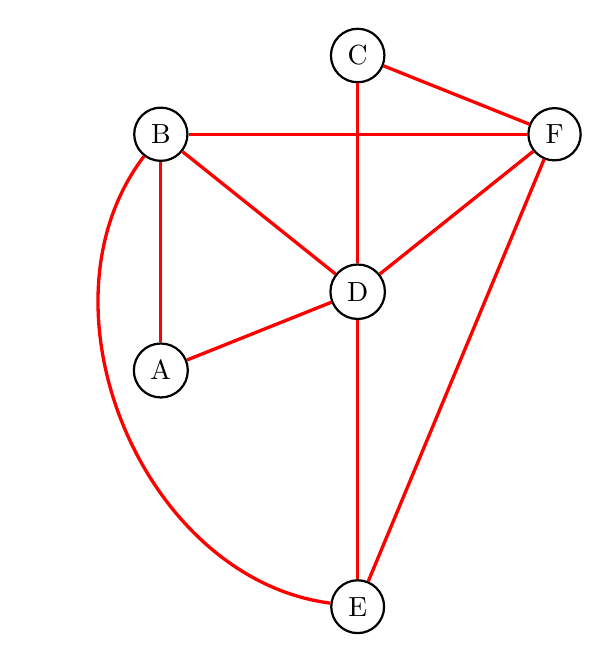
\begin{tikzpicture}
\begin{scope}[every node/.style={circle,thick,draw}]
    \node (A) at (0,0) {A};
    \node (B) at (0,3) {B};
    \node (C) at (2.5,4) {C};
    \node (D) at (2.5,1) {D};
    \node (E) at (2.5,-3) {E};
    \node (F) at (5,3) {F} ;
\end{scope}

\begin{scope}[>={Stealth[black]},
              every node/.style={fill=white,circle},
              every edge/.style={draw=red,very thick}]
    \path [-] (C) edge (D);
    \path [-] (D) edge (E);
    \path [-] (C) edge (F);
    \path [-] (F) edge (E);
    \path [-] (F) edge (D);
    \path [-] (B) edge (D);
    \path [-] (F) edge (B);
    \path [-] (E) edge[bend left=60] (B);
    \path [-] (A) edge (B); 
    \path [-] (D) edge (A); 
\end{scope}
\end{tikzpicture}
\hspace{50pt}
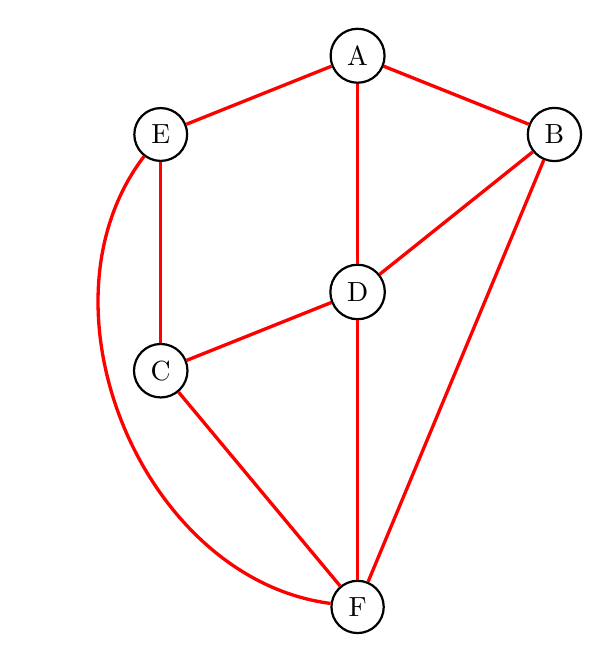
\begin{tikzpicture}
\begin{scope}[every node/.style={circle,thick,draw}]
    \node (A) at (0,0) {C};
    \node (B) at (0,3) {E};
    \node (C) at (2.5,4) {A};
    \node (D) at (2.5,1) {D};
    \node (E) at (2.5,-3) {F};
    \node (F) at (5,3) {B} ;
\end{scope}

\begin{scope}[>={Stealth[black]},
              every node/.style={fill=white,circle},
              every edge/.style={draw=red,very thick}]
    \path [-] (A) edge (B);
    \path [-] (B) edge (C);
    \path [-] (A) edge (D);
    \path [-] (D) edge (C);
    \path [-] (A) edge (E);
    \path [-] (D) edge (E);
    \path [-] (D) edge (F);
    \path [-] (C) edge (F);
    \path [-] (E) edge (F); 
    \path [-] (B) edge[bend right=60] (E); 
\end{scope}
\end{tikzpicture}}
\end{center}

\newpage

\item[2.] Let $G,H,K$ be simple graphs.
\begin{enumerate}
    \item If $G\cong H$, prove that $\ba{G}\cong\ba{H}$.
    \item If $K\subseteq G$ and $V(K)=V(G)$, prove that $\ba{G}\subseteq{\ba{K}}$ \textcolor{blue}{(NOTE: corrected from original)}
\end{enumerate}

\item[3.] Let $G$ be a simple graph with incidence matrix $M$.
\begin{enumerate}
    \item What meanings to the entries in position $(i,j)$ of $MM^T$ and $M^TM$ have in terms of the edges and vertices of $G$? I.e. what does entry $(i,j)$ tell you about $G$?
    \item Prove that all diagonal entries of $M^TM$ are 2.
\end{enumerate}

\item[4.] Prove that every group of six people contains either a set of three people who all know each other or a set of three people who all do not know each other.

\item[5.] Prove that the Petersen graph has no cycle of length 7 (i.e. a subgraph that is a cycle consisting of exactly 7 vertices).

\end{enumerate}


\end{document}
